\documentclass[11pt,a4paper]{article}
%%%%%%%%%%%%%%%%%%%%%%%%% Credit %%%%%%%%%%%%%%%%%%%%%%%%

% template ini dibuat oleh martin.manullang@if.itera.ac.id untuk dipergunakan oleh seluruh sivitas akademik itera.

%%%%%%%%%%%%%%%%%%%%%%%%% PACKAGE starts HERE %%%%%%%%%%%%%%%%%%%%%%%%
\usepackage{graphicx}
\usepackage{caption}
\usepackage{microtype}
\usepackage{lmodern}
\captionsetup[table]{name=Tabel}
\captionsetup[figure]{name=Gambar}
\usepackage{tabulary}
\usepackage{minted}
\usepackage{amsmath}
\usepackage{fancyhdr}
\usepackage{amssymb}
\usepackage{amsthm}
\usepackage{placeins}
\usepackage{amsfonts}
\usepackage{graphicx}
\usepackage[all]{xy}
\usepackage{tikz}
\usepackage{verbatim}
\usepackage[left=2cm,right=2cm,top=3cm,bottom=2.5cm]{geometry}
\usepackage{hyperref}
\hypersetup{
    colorlinks,
    linkcolor={red!50!black},
    citecolor={blue!50!black},
    urlcolor={blue!80!black}
}
\usepackage{caption}
\usepackage{subcaption}
\usepackage{multirow}
\usepackage{psfrag}
\usepackage[T1]{fontenc}
\usepackage[scaled]{beramono}
% Enable inserting code into the document
\usepackage{listings}
\usepackage{xcolor} 
% custom color & style for listing
\definecolor{codegreen}{rgb}{0,0.6,0}
\definecolor{codegray}{rgb}{0.5,0.5,0.5}
\definecolor{codepurple}{rgb}{0.58,0,0.82}
\definecolor{backcolour}{rgb}{0.95,0.95,0.92}
\definecolor{LightGray}{gray}{0.9}
\lstdefinestyle{mystyle}{
	backgroundcolor=\color{backcolour},   
	commentstyle=\color{green},
	keywordstyle=\color{codegreen},
	numberstyle=\tiny\color{codegray},
	stringstyle=\color{codepurple},
	basicstyle=\ttfamily\footnotesize,
	breakatwhitespace=false,         
	breaklines=true,                 
	captionpos=b,                    
	keepspaces=true,                 
	numbers=left,                    
	numbersep=5pt,                  
	showspaces=false,                
	showstringspaces=false,
	showtabs=false,                  
	tabsize=2
}
\lstset{style=mystyle}
\renewcommand{\lstlistingname}{Kode}
%%%%%%%%%%%%%%%%%%%%%%%%% PACKAGE ends HERE %%%%%%%%%%%%%%%%%%%%%%%%


%%%%%%%%%%%%%%%%%%%%%%%%% Data Diri %%%%%%%%%%%%%%%%%%%%%%%%
\newcommand{\student}{\textbf{Reynaldi Cristian Simamora (122140116)}}
\newcommand{\course}{\textbf{Sistem Teknologi Multimedia (IF25-40305)}}
\newcommand{\assignment}{\textbf{Worksheet 1: Setup Python Environment untuk Multimedia}}

%%%%%%%%%%%%%%%%%%% using theorem style %%%%%%%%%%%%%%%%%%%%
\newtheorem{thm}{Theorem}
\newtheorem{lem}[thm]{Lemma}
\newtheorem{defn}[thm]{Definition}
\newtheorem{exa}[thm]{Example}
\newtheorem{rem}[thm]{Remark}
\newtheorem{coro}[thm]{Corollary}
\newtheorem{quest}{Question}[section]
%%%%%%%%%%%%%%%%%%%%%%%%%%%%%%%%%%%%%%%%
\usepackage{lipsum}%% a garbage package you don't need except to create examples.
\usepackage{fancyhdr}
\pagestyle{fancy}
\lhead{Nama Mahasiswa di Header (NIM Mahasiswa di Header)}
\rhead{ \thepage}
\cfoot{\textbf{Worksheet 1: Setup Python Environment untuk Multimedia}}
\renewcommand{\headrulewidth}{0.4pt}
\renewcommand{\footrulewidth}{0.4pt}

%%%%%%%%%%%%%%  Shortcut for usual set of numbers  %%%%%%%%%%%

\newcommand{\N}{\mathbb{N}}
\newcommand{\Z}{\mathbb{Z}}
\newcommand{\Q}{\mathbb{Q}}
\newcommand{\R}{\mathbb{R}}
\newcommand{\C}{\mathbb{C}}
\setlength\headheight{14pt}

%%%%%%%%%%%%%%%%%%%%%%%%%%%%%%%%%%%%%%%%%%%%%%%%%%%%%%%555
\begin{document}
\thispagestyle{empty}
\begin{center}
	
\includegraphics[scale = 0.15]{Figure/ifitera-header.png}
	\vspace{0.1cm}
\end{center}
\noindent
\rule{17cm}{0.2cm}\\[0.3cm]
Nama: \student \hfill Tugas Ke: \assignment\\[0.1cm]
Mata Kuliah: \course \hfill Tanggal: \today\\
\rule{17cm}{0.05cm}
\vspace{0.1cm}



%%%%%%%%%%%%%%%%%%%%%%%%%%%%%%%%%%%%%%%%%%%%% BODY DOCUMENT %%%%%%%%%%%%%%%%%%%%%%%%%%%%%%%%%%%%%%%%%%%%%
\section{Tujuan Pembelajaran}
Setelah menyelesaikan worksheet ini, mahasiswa diharapkan mampu:
\begin{itemize}
    \item Memahami pentingnya manajemen environment Python untuk pengembangan multimedia
    \item Menginstall dan mengkonfigurasi Python environment menggunakan conda, venv, atau uv
    \item Menginstall library-library Python yang diperlukan untuk multimedia processing
    \item Memverifikasi instalasi dengan mengimpor dan menguji library multimedia
    \item Mendokumentasikan proses konfigurasi dan hasil pengujian dalam format \LaTeX
\end{itemize}

\section{Latar Belakang}
Python telah menjadi bahasa pemrograman yang sangat populer untuk multimedia processing karena memiliki ekosistem library yang sangat kaya. Namun, untuk dapat bekerja dengan multimedia secara efektif, kita perlu mengatur environment Python dengan benar dan menginstall library-library yang tepat.

Manajemen environment Python sangat penting untuk:
\begin{itemize}
    \item Menghindari konflik antar library (dependency conflict)
    \item Memastikan reproducibility dari project
    \item Memudahkan kolaborasi antar developer
    \item Memisahkan project yang berbeda dengan requirement yang berbeda
\end{itemize}

\section{Instruksi Tugas}

\subsection{Persiapan}
\textbf{Sebelum memulai, pastikan Anda telah:}
\begin{itemize}
    \item Menginstall Python 3.8 atau lebih baru di sistem Anda
    \item Memilih salah satu tool manajemen environment: \textbf{conda}, \textbf{venv}, atau \textbf{uv}
    \item Membuka terminal/command prompt
    \item Menyiapkan dokumen \LaTeX\ ini untuk dokumentasi
\end{itemize}

\subsection{Bagian 1: Membuat Environment Python}
Pilih \textbf{SALAH SATU} dari tiga opsi berikut dan ikuti langkah-langkahnya:

\subsubsection{Opsi 1: Menggunakan Conda (Direkomendasikan untuk pemula)}
Jalankan perintah berikut di terminal:

\begin{lstlisting}[language=bash, caption=Membuat environment dengan Conda]
# Membuat environment baru dengan nama 'multimedia'
conda create -n multimedia python=3.11

# Mengaktifkan environment
conda activate multimedia

# Verifikasi environment aktif
conda info --envs
\end{lstlisting}

\subsubsection{Opsi 2: Menggunakan venv (Built-in Python)}
\begin{lstlisting}[language=bash, caption=Membuat environment dengan venv]
# Membuat environment baru
python3 -m venv multimedia-env

# Mengaktifkan environment (Linux/Mac)
source multimedia-env/bin/activate

# Mengaktifkan environment (Windows)
# multimedia-env\Scripts\activate

# Verifikasi environment aktif
which python
\end{lstlisting}

\subsubsection{Opsi 3: Menggunakan uv (Modern dan cepat)}
\begin{lstlisting}[language=bash, caption=Membuat environment dengan uv]
# Install uv terlebih dahulu jika belum ada
# pip install uv

# Membuat environment baru
uv venv multimedia-uv

# Mengaktifkan environment (Linux/Mac)
source multimedia-uv/bin/activate

# Mengaktifkan environment (Windows)
# multimedia-uv\Scripts\activate

# Verifikasi environment aktif
which python
\end{lstlisting}

\textbf{Dokumentasikan di sini:}
\begin{itemize}
    \item Tool manajemen environment yang Anda pilih: \textbf{conda}
    \item Screenshot atau copy-paste output dari perintah verifikasi environment
\end{itemize}

\textbf{Output : verifikasi instalasi}
\begin{lstlisting}[caption=Output verifikasi instalasi Environment Melalui Conda]
D:\Users\Downloads\Worksheet 1 (1)\Worksheet 1>conda activate multimedia

(multimedia) D:\Users\Downloads\Worksheet 1 (1)\Worksheet 1>conda info --envs

# conda environments:
#
base                   C:\ProgramData\miniconda3
handson                C:\Users\ANSEN\.conda\envs\handson
multimedia           * C:\Users\ANSEN\.conda\envs\multimedia
myenv                  C:\Users\ANSEN\.conda\envs\myenv

(multimedia) D:\Users\Downloads\Worksheet 1 (1)\Worksheet 1>
\end{lstlisting}

\subsection{Bagian 2: Instalasi Library Multimedia}
Setelah environment aktif, install library-library berikut:

\subsubsection{Library Audio Processing}
\begin{lstlisting}[language=bash, caption=Instalasi library audio]
# Untuk conda:
conda install -c conda-forge librosa soundfile scipy

# Untuk pip (venv/uv):
pip install librosa soundfile scipy
\end{lstlisting}

\subsubsection{Library Image Processing}
\begin{lstlisting}[language=bash, caption=Instalasi library image]
# Untuk conda:
conda install -c conda-forge opencv pillow scikit-image matplotlib

# Untuk pip (venv/uv):
pip install opencv-python pillow scikit-image matplotlib
\end{lstlisting}

\subsubsection{Library Video Processing}
\begin{lstlisting}[language=bash, caption=Instalasi library video]
# Untuk conda:
conda install -c conda-forge ffmpeg
pip install moviepy

# Untuk pip (venv/uv):
pip install moviepy
\end{lstlisting}

\subsubsection{Library General Purpose}
\begin{lstlisting}[language=bash, caption=Instalasi library umum]
# Untuk conda:
conda install numpy pandas jupyter

# Untuk pip (venv/uv):
pip install numpy pandas jupyter
\end{lstlisting}

\textbf{Dokumentasikan di sini:}
\begin{itemize}
    \item Perintah instalasi yang Anda gunakan
    \begin{lstlisting}[language=bash, caption=Instalasi library video]
        //Saya menggunakan instalansi via conda untuk keempat library di atas
        conda install -c conda --forge librosa soundfile scipy
        conda install -c conda-forge opencv pillow scikit-image matplotlib
        conda install -c conda-forge ffmpeg
        conda install numpy pandas jupyter
    \end{lstlisting}
    \item Screenshot proses instalasi atau output sukses
    \begin{lstlisting}[language=bash, caption=Output instalansi library]
(multimedia) D:\Users\Downloads\Worksheet 1 (1)\Worksheet 1>conda install -c conda-forge librosa soundfile scipy
Retrieving notices: done
Channels:     
 - conda-forge
 - defaults   
Platform: win-64
Collecting package metadata (repodata.json): done
Solving environment: done
==> WARNING: A newer version of conda exists. <==
    current version: 25.3.1
    latest version: 25.7.0
Please update conda by running
    $ conda update -n base -c defaults conda

## Package Plan ##

  environment location: C:\Users\ANSEN\.conda\envs\multimedia

  added / updated specs:
    - librosa
    - scipy
    - soundfile
The following packages will be downloaded:

    package                    |            build
    ---------------------------|-----------------
    ca-certificates-2025.8.3   |       h4c7d964_0         151 KB  conda-forge
    cpython-3.11.13            |  py311hd8ed1ab_0          46 KB  conda-forge
    importlib-metadata-8.7.0   |     pyhe01879c_1          34 KB  conda-forge
    jsonschema-with-format-nongpl-4.25.1|       he01879c_0           5 KB  conda-forge
    ....                       |    ....................
    tomli-2.2.1                |     pyhe01879c_2          21 KB  conda-forge
    zipp-3.23.0                |     pyhd8ed1ab_0          22 KB  conda-forge
    ------------------------------------------------------------
                                           Total:       137.6 MB
The following NEW packages will be INSTALLED:

  cpython            conda-forge/noarch::cpython-3.11.13-py311hd8ed1ab_0
  importlib-metadata conda-forge/noarch::importlib-metadata-8.7.0-pyhe01879c_1
  jsonschema-with-f~ conda-forge/noarch::jsonschema-with-format-nongpl-4.25.1-he01879c_0
  jupyter_client     conda-forge/noarch::jupyter_client-8.6.3-pyhd8ed1ab_1
  ....               ...........................
  zipp               conda-forge/noarch::zipp-3.23.0-pyhd8ed1ab_0

The following packages will be UPDATED:

  ca-certificates    pkgs/main/win-64::ca-certificates-202~ --> conda-forge/noarch::ca-certificates-2025.8.3-h4c7d964_0
  openssl              pkgs/main::openssl-3.0.17-h35632f6_0 --> conda-forge::openssl-3.5.2-h725018a_0
  scipy                      pypi/pypi::scipy-1.16.1-pypi_0 --> conda-forge/win-64::scipy-1.16.2-py311h9a1c30b_0

The following packages will be SUPERSEDED by a higher-priority channel:

  jupyterlab             pypi/pypi::jupyterlab-4.4.7-pypi_0 --> conda-forge/noarch::jupyterlab-4.4.7-pyhd8ed1ab_0


Proceed ([y]/n)? y

Downloading and Extracting Packages:

Preparing transaction: done
Verifying transaction: done
Executing transaction: done

(multimedia) D:\Users\Downloads\Worksheet 1 (1)\Worksheet 1>conda install -c conda-forge opencv pillow scikit-image matplotlib
Channels:
 - conda-forge
 - defaults
Platform: win-64
Collecting package metadata (repodata.json): done
Solving environment: done

==> WARNING: A newer version of conda exists. <==
    current version: 25.3.1
    latest version: 25.7.0

Please update conda by running

    $ conda update -n base -c defaults conda

## Package Plan ##

  environment location: C:\Users\ANSEN\.conda\envs\multimedia

  added / updated specs:
    - matplotlib
    - opencv
    - pillow
    - scikit-image

The following packages will be downloaded:

    package                    |            build
    ---------------------------|-----------------
    _libavif_api-1.3.0         |       h57928b3_2          10 KB  conda-forge
    aom-3.9.1                  |       he0c23c2_0         1.9 MB  conda-forge
    blosc-1.21.6               |       h4190f5b_0         100 KB
    brotli-1.0.9               |       hcfcfb64_9          20 KB  conda-forge
    ....                       |       ...
    ------------------------------------------------------------
                                           Total:       375.3 MB

The following NEW packages will be INSTALLED:

  _libavif_api       conda-forge/win-64::_libavif_api-1.3.0-h57928b3_2
  aom                conda-forge/win-64::aom-3.9.1-he0c23c2_0
  ....               ...........................
  1-h2f0f97f_3
  zlib-ng            conda-forge/win-64::zlib-ng-2.0.7-hcfcfb64_0
  zstd               pkgs/main/win-64::zstd-1.5.6-h8880b57_0

Proceed ([y]/n)? y

Downloading and Extracting Packages:
qtwebengine-6.7.3    | 146.1 MB  | ###################6                                                                                                                 |  15%  
opencv-4.10.0        | 40.0 MB   | ###########################################################################9                                                         |  58%  
qtwebengine-6.7.3    | 146.1 MB  | ###################7                                                                                                                 |  15%  
opencv-4.10.0        | 40.0 MB   | ############################################################################1                                                        |  58%  
qtwebengine-6.7.3    | 146.1 MB  | ###################7                                                                                                                 |  15%  

Preparing transaction: done
Verifying transaction: done
Executing transaction: done

(multimedia) D:\Users\Downloads\Worksheet 1 (1)\Worksheet 1>conda install -c conda-forge ffmpeg
Channels:
 - conda-forge
 - defaults
Platform: win-64
Collecting package metadata (repodata.json): done
Solving environment: done


==> WARNING: A newer version of conda exists. <==
    current version: 25.3.1
    latest version: 25.7.0

Please update conda by running

    $ conda update -n base -c defaults conda

## Package Plan ##

  environment location: C:\Users\ANSEN\.conda\envs\multimedia

  added / updated specs:
    - ffmpeg


The following packages will be downloaded:

    package                    |            build
    ---------------------------|-----------------
    ffmpeg-4.3.1               |       ha925a31_0        26.2 MB  conda-forge
    ------------------------------------------------------------
                                           Total:        26.2 MB
The following NEW packages will be INSTALLED:

  ffmpeg             conda-forge/win-64::ffmpeg-4.3.1-ha925a31_0
Proceed ([y]/n)? y
Downloading and Extracting Packages:

Preparing transaction: done
Verifying transaction: done
Executing transaction: done

(multimedia) D:\Users\Downloads\Worksheet 1 (1)\Worksheet 1>conda install numpy pandas jupyter
Channels:
 - defaults
Platform: win-64
Collecting package metadata (repodata.json): done
Solving environment: done

==> WARNING: A newer version of conda exists. <==
    current version: 25.3.1
    latest version: 25.7.0

Please update conda by running

    $ conda update -n base -c defaults conda

## Package Plan ##

  environment location: C:\Users\ANSEN\.conda\envs\multimedia

  added / updated specs:
    - jupyter
    - numpy
    - pandas


The following packages will be downloaded:

    package                    |            build
    ---------------------------|-----------------
    asttokens-3.0.0            |  py311haa95532_0          49 KB
    bottleneck-1.4.2           |  py311h57dcf0c_0         146 KB
    ca-certificates-2025.9.9   |       haa95532_0         127 KB
    .....                      |    .....................
    widgetsnbextension-4.0.13  |  py311haa95532_0         949 KB
    zeromq-4.3.5               |       h6c54ac7_1         4.0 MB
    ------------------------------------------------------------
                                           Total:       212.6 MB

The following NEW packages will be INSTALLED:

  asttokens          pkgs/main/win-64::asttokens-3.0.0-py311haa95532_0
  blas               pkgs/main/win-64::blas-1.0-mkl
  bottleneck         pkgs/main/win-64::bottleneck-1.4.2-py311h57dcf0c_0
  ...                ...........................
  widgetsnbextension pkgs/main/win-64::widgetsnbextension-4.0.13-py311haa95532_0
  zeromq             pkgs/main/win-64::zeromq-4.3.5-h6c54ac7_1

The following packages will be REMOVED:

  libblas-3.9.0-35_h5709861_mkl
  libcblas-3.9.0-35_h2a3cdd5_mkl
  liblapack-3.9.0-35_hf9ab0e9_mkl

The following packages will be UPDATED:

  ca-certificates    conda-forge/noarch::ca-certificates-2~ --> pkgs/main/win-64::ca-certificates-2025.9.9-haa95532_0
  mkl                 conda-forge::mkl-2024.2.2-h57928b3_16 --> pkgs/main::mkl-2025.0.0-h5da7b33_930
  tbb                 conda-forge::tbb-2021.13.0-h18a62a1_3 --> pkgs/main::tbb-2022.0.0-h214f63a_0

The following packages will be SUPERSEDED by a higher-priority channel:

  llvm-openmp        conda-forge::llvm-openmp-20.1.8-hfa2b~ --> pkgs/main::llvm-openmp-20.1.8-h29ce207_0
  numpy              conda-forge::numpy-2.3.3-py311h80b3fa~ --> pkgs/main::numpy-2.3.3-py311hc2e1e29_0
  scipy              conda-forge::scipy-1.16.2-py311h9a1c3~ --> pkgs/main::scipy-1.16.1-py311h86a6471_0

The following packages will be DOWNGRADED:

  setuptools                         78.1.1-py311haa95532_0 --> 72.1.0-py311haa95532_0

Proceed ([y]/n)?


Downloading and Extracting Packages:
mkl-2025.0.0         | 104.7 MB  | #################################################################################################################################### | 100%  
scipy-1.16.1         | 28.1 MB   | #################################################################################################################################### | 100%  
pandoc-2.12          | 14.6 MB   | #################################################################################################################################### | 100%  
pandas-2.3.2         | 14.3 MB   | #################################################################################################################################### | 100%  
notebook-7.4.5       | 11.0 MB   | #################################################################################################################################### | 100%  
numpy-base-2.3.3     | 9.7 MB    | #################################################################################################################################### | 100%  
zeromq-4.3.5         | 4.0 MB    | #################################################################################################################################### | 100%  
debugpy-1.8.16       | 3.5 MB    | #################################################################################################################################### | 100%  
pyqt-6.7.1           | 3.5 MB    | #################################################################################################################################### | 100%  
setuptools-72.1.0    | 3.0 MB    | #################################################################################################################################### | 100%  
pygments-2.19.1      | 2.2 MB    | #################################################################################################################################### | 100%  
intel-openmp-2025.0. | 2.1 MB    | #################################################################################################################################### | 100%  
ipython-9.1.0        | 1.2 MB    | #################################################################################################################################### | 100%  
jedi-0.19.2          | 1.2 MB    | #################################################################################################################################### | 100%  
tbb-devel-2022.0.0   | 1.1 MB    | #################################################################################################################################### | 100%  
widgetsnbextension-4 | 949 KB    | #################################################################################################################################### | 100%  
prompt-toolkit-3.0.4 | 746 KB    | #################################################################################################################################### | 100%  
sip-6.10.0           | 718 KB    | #################################################################################################################################### | 100%  
psutil-7.0.0         | 571 KB    | #################################################################################################################################### | 100%  
                                                                                                                                                                                
Preparing transaction: done
Verifying transaction: done
Executing transaction: done
    \end{lstlisting}
    \item Daftar library yang berhasil diinstall dengan versinya

\end{itemize}

\subsection{Bagian 3: Verifikasi Instalasi}
Buat file Python sederhana untuk menguji semua library yang telah diinstall:
\begin{lstlisting}[language=bash, caption = Verifikasi Versi Library yang Diinstal]
(multimedia) D:\Users\Downloads\Worksheet 1 (1)\Worksheet 1>conda list | findstr "librosa soundfile scipy opencv pillow scikit-image matplotlib ffmpeg jupyter"
ffmpeg                    4.3.1                ha925a31_0    conda-forge
imageio-ffmpeg            0.6.0                    pypi_0    pypi       
jupyter                   1.1.1           py311haa95532_0
jupyter-lsp               2.3.0                    pypi_0    pypi       
jupyter_client            8.6.3              pyhd8ed1ab_1    conda-forge
jupyter_console           6.6.3           py311haa95532_0
jupyter_core              5.8.1              pyh5737063_0    conda-forge
jupyter_events            0.12.0             pyh29332c3_0    conda-forge
jupyter_server            2.17.0             pyhcf101f3_0    conda-forge
jupyter_server_terminals  0.5.3              pyhd8ed1ab_1    conda-forge
jupyterlab                4.4.7              pyhd8ed1ab_0    conda-forge
jupyterlab_pygments       0.3.0              pyhd8ed1ab_2    conda-forge
jupyterlab_server         2.27.3             pyhd8ed1ab_1    conda-forge
jupyterlab_widgets        3.0.15          py311haa95532_0
librosa                   0.11.0                   pypi_0    pypi       
matplotlib                3.10.6          py311h1ea47a8_1    conda-forge
matplotlib-base           3.10.6          py311h43afe63_0
matplotlib-inline         0.1.7                    pypi_0    pypi
opencv                    4.10.0          py311h28596fa_7
opencv-python             4.12.0.88                pypi_0    pypi
pillow                    11.3.0          py311hb328d1f_0
scikit-image              0.25.2          py311h11fd7f3_2    conda-forge
scipy                     1.16.1          py311h86a6471_0
soundfile                 0.13.1                   pypi_0    pypi
\end{lstlisting}

\textbf{Jalankan script dan dokumentasikan hasilnya:}

\subsection{Bagian 4: Simple Test dengan Sample Code}
Buat dan jalankan contoh sederhana untuk setiap kategori multimedia:

\subsubsection{Test Audio Processing}
\begin{lstlisting}[language=Python, caption=Test audio processing sederhana]
import numpy as np
import matplotlib.pyplot as plt

# Generate simple sine wave
duration = 2  # seconds
sample_rate = 44100
frequency = 440  # A4 note

t = np.linspace(0, duration, int(sample_rate * duration))
audio_signal = np.sin(2 * np.pi * frequency * t)

# Plot waveform
plt.figure(figsize=(10, 4))
plt.plot(t[:1000], audio_signal[:1000])  # Plot first 1000 samples
plt.title('Sine Wave (440 Hz)')
plt.xlabel('Time (s)')
plt.ylabel('Amplitude')
plt.grid(True)
plt.savefig('sine_wave_test.png', dpi=150, bbox_inches='tight')
plt.show()

print(f"Generated {duration}s sine wave at {frequency}Hz")
print(f"Sample rate: {sample_rate}Hz")
print(f"Total samples: {len(audio_signal)}")
\end{lstlisting}

\subsubsection{Test Image Processing}
\begin{lstlisting}[language=Python, caption=Test image processing sederhana]
import numpy as np
import matplotlib.pyplot as plt
from PIL import Image

# Create a simple test image
width, height = 400, 300
image = np.zeros((height, width, 3), dtype=np.uint8)

# Add some patterns
image[:, :width//3, 0] = 255  # Red section
image[:, width//3:2*width//3, 1] = 255  # Green section
image[:, 2*width//3:, 2] = 255  # Blue section

# Add a white circle in the center
center_x, center_y = width//2, height//2
radius = 50
Y, X = np.ogrid[:height, :width]
mask = (X - center_x)**2 + (Y - center_y)**2 <= radius**2
image[mask] = [255, 255, 255]

# Display and save
plt.figure(figsize=(8, 6))
plt.imshow(image)
plt.title('Test Image with RGB Stripes and White Circle')
plt.axis('off')
plt.savefig('test_image.png', dpi=150, bbox_inches='tight')
plt.show()

print(f"Created test image: {width}x{height} pixels")
print(f"Image shape: {image.shape}")
print(f"Image dtype: {image.dtype}")
\end{lstlisting}

\textbf{Dokumentasikan hasil eksekusi:}
\begin{itemize}
    \item Screenshot output dari kedua script di atas
    \item Gambar yang dihasilkan (sine\_wave\_test.png dan test\_image.png)\\    
    \item Error message jika ada dan cara mengatasinya\\
    \textbf{[Deskripsi masalah dan solusi di sini]}
\end{itemize}

\section{Bagian Laporan}

\subsection{Output Verifikasi Instalasi}
\textbf{Copy-paste output lengkap dari script \texttt{test\_multimedia.py} di sini:}
\begin{lstlisting}[language=bash, caption=Output verifikasi instalasi]
# Saya menjalankan script test audio dan image di atas file ipynb
# Output dari script test audio (sine_wave_test.png)

Generated 2s sine wave at 440Hz
Sample rate: 44100Hz
Total samples: 88200

# Output dari script test image (test_image.png)

Created test image: 400x300 pixels
Image shape: (300, 400, 3)
Image dtype: uint8
\end{lstlisting}

\subsection{Screenshot Hasil Test}
\textbf{Sisipkan screenshot atau gambar hasil dari:}
\begin{itemize}
    \item Terminal/command prompt yang menunjukkan environment aktif\\\\
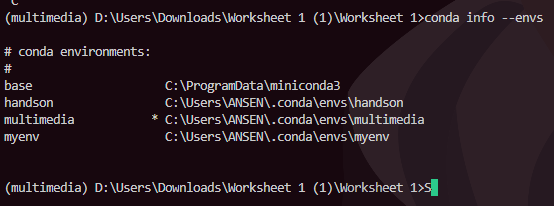
\includegraphics[width=0.8\textwidth]{Figure/activate_environment.png}\\
    \item Output dari script test audio (sine wave plot)\\\\
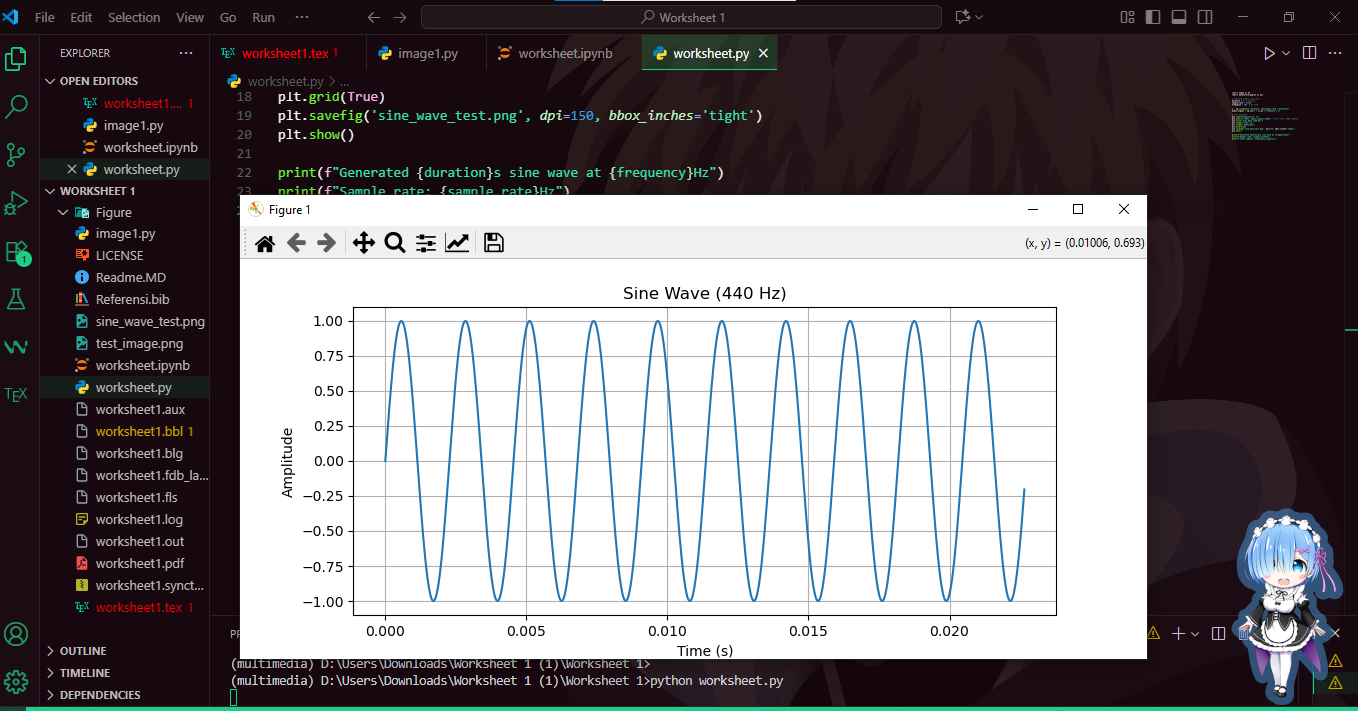
\includegraphics[width=0.8\textwidth]{Figure/waveform.png}\\
    \item Output dari script test image (RGB stripes dengan circle)\\\\
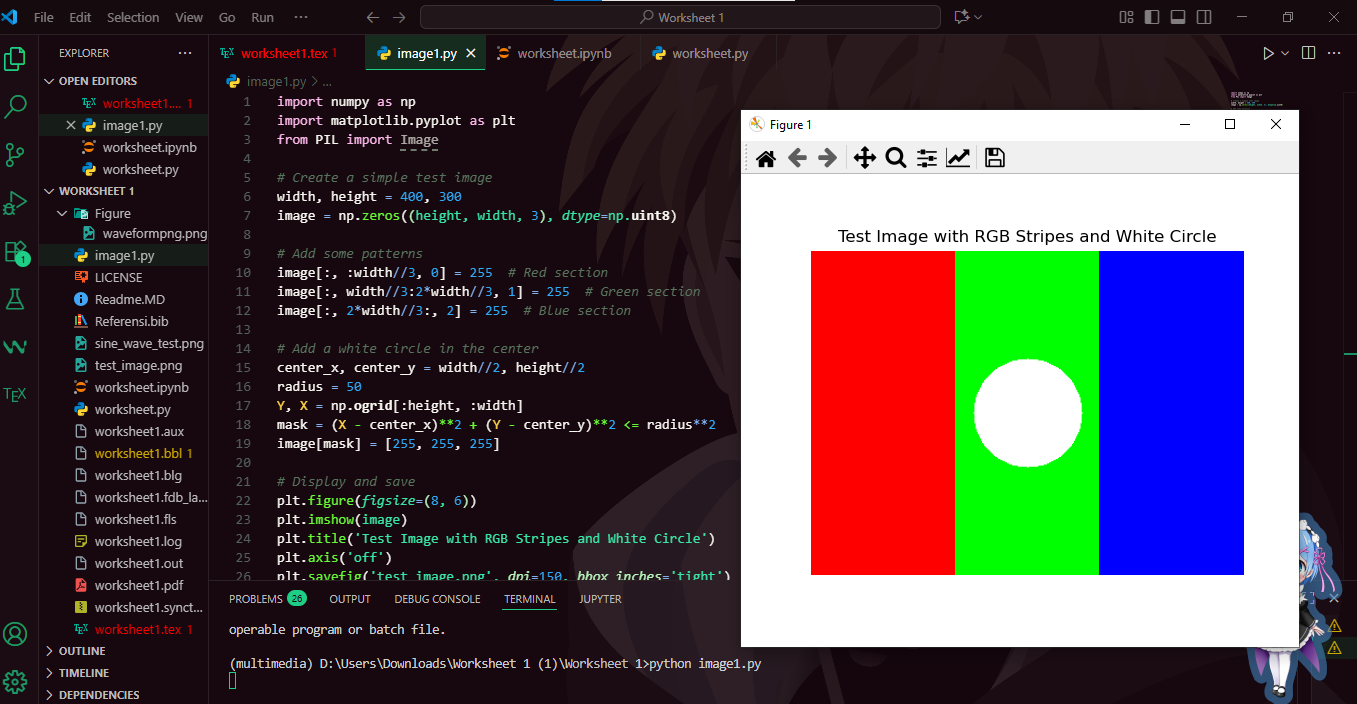
\includegraphics[width=0.8\textwidth]{Figure/rgbtest.png}\\
\end{itemize}

\subsection{Analisis dan Refleksi}
\textbf{Jawab pertanyaan berikut:}

\begin{enumerate}
    \item \textbf{Mengapa penting menggunakan environment terpisah untuk project multimedia?}
    
    Penggunaan environment terpisah sangat penting karena project multimedia biasanya membutuhkan banyak library dengan dependensi yang kompleks, bahkan terkadang berbeda versi antara satu project dengan project lain. Dengan membuat environment khusus, kita dapat menghindari benturan versi library, menjaga stabilitas project, serta mempermudah replikasi di komputer lain tanpa merusak konfigurasi global Python.
    
    \item \textbf{Apa perbedaan utama antara conda, venv, dan uv? Mengapa Anda memilih tool yang Anda gunakan?}
    
    \texttt{conda} merupakan package manager sekaligus environment manager yang mampu mengatur library Python maupun non-Python (misalnya \textit{ffmpeg} atau \textit{OpenCV} berbasis C++). \texttt{venv} hanya membuat virtual environment Python sederhana, tanpa manajemen dependensi tingkat lanjut. Sedangkan \texttt{uv} lebih modern dan berfokus pada performa instalasi yang lebih cepat, tetapi ekosistemnya masih relatif baru. Pada project ini saya memilih menggunakan \texttt{conda} karena lebih stabil dalam menangani dependensi multimedia yang kompleks.
    
    \item \textbf{Library mana yang paling sulit diinstall dan mengapa?}
    
    Library yang paling sulit diinstall adalah \texttt{librosa}, karena selain membutuhkan \texttt{numpy} dan \texttt{scipy}, library ini juga bergantung pada \texttt{soundfile} yang membutuhkan dukungan dari \texttt{libsndfile} (library non-Python). Hal ini sering menyebabkan error apabila instalasi hanya menggunakan \texttt{pip} tanpa dependensi sistem yang lengkap. Dengan \texttt{conda}, masalah ini lebih mudah teratasi karena paket biner sudah tersedia.
    
    \item \textbf{Bagaimana cara mengatasi masalah dependency conflict jika terjadi?}
    
    Cara yang umum dilakukan adalah dengan memperbarui atau menurunkan versi library sesuai rekomendasi dari error log. Selain itu, saya juga bisa mencoba membuat environment baru yang lebih bersih, kemudian menginstal library satu per satu dengan urutan yang benar. Jika library tidak tersedia di conda, saya melengkapinya dengan \texttt{pip install} di dalam environment tersebut. Strategi ini efektif mengurangi potensi konflik dependensi.
    
    \item \textbf{Jelaskan fungsi dari masing-masing library yang berhasil Anda install!}
    
    \begin{itemize}
        \item \textbf{librosa}: Digunakan untuk analisis dan pemrosesan sinyal audio, seperti ekstraksi fitur (MFCC, mel-spectrogram).
        \item \textbf{soundfile}: Membaca dan menulis file audio dengan format \texttt{.wav}, \texttt{.flac}, dan lainnya.
        \item \textbf{scipy}: Library sains yang mendukung operasi matematika lanjutan, optimasi, dan pemrosesan sinyal.
        \item \textbf{opencv}: Pemrosesan citra dan video, termasuk deteksi objek, filtering, dan transformasi.
        \item \textbf{pillow}: Manipulasi gambar (membaca, menulis, editing gambar format umum).
        \item \textbf{scikit-image}: Analisis citra ilmiah seperti segmentasi, filtering, dan feature extraction.
        \item \textbf{matplotlib}: Visualisasi data dalam bentuk grafik, plot, maupun gambar.
        \item \textbf{ffmpeg}: Toolkit multimedia untuk konversi, decoding, dan encoding file audio-video.
        \item \textbf{jupyter}: Lingkungan interaktif berbasis notebook untuk eksperimen dan dokumentasi kode Python.
    \end{itemize}
\end{enumerate}


\subsection{Troubleshooting}
\textbf{Dokumentasikan masalah yang Anda hadapi (jika ada) dan cara mengatasinya:}

\begin{itemize}
    \item \textbf{Masalah 1:} Saat menginstal library multimedia menggunakan \texttt{pip} di dalam environment conda yang sudah aktif, proses instalasi gagal karena beberapa dependensi non-Python (misalnya \texttt{libsndfile} untuk \texttt{soundfile}) tidak terpenuhi. Hal ini menyebabkan error dan library tidak dapat digunakan.
    
    \textbf{Solusi:} Menggunakan \texttt{conda install -c conda-forge <nama\_library>} untuk menginstal library tersebut. Dengan conda, dependensi non-Python juga akan terpasang otomatis sehingga instalasi berhasil tanpa error.
    
    \item \textbf{Masalah 2:} Saat menyusun laporan menggunakan LaTeX, proses kompilasi membutuhkan waktu lama dan muncul error \texttt{Package caption: Unused \textbackslash captionsetup[table]}. Error ini muncul karena terdapat perintah konfigurasi caption untuk \texttt{table}, sementara di dokumen tidak ada environment tabel yang aktif.
    
    \textbf{Solusi:} Menghapus atau menonaktifkan baris \texttt{\textbackslash captionsetup[table]\{...\}} jika memang tidak menggunakan tabel. Alternatifnya, jika ingin tetap mendukung caption untuk tabel, pastikan ada lingkungan \texttt{table} yang sesuai di dokumen. Dengan cara ini error dapat diatasi dan proses kompilasi berjalan lebih cepat.
\end{itemize}

\section{Export Environment untuk Reproduksi}
Sebagai langkah terakhir, export environment Anda agar dapat direproduksi:

\subsection{Untuk Conda}
\begin{lstlisting}[language=bash, caption=Export conda environment]
conda env export > environment.yml
\end{lstlisting}

\subsection{Untuk venv/uv}
\begin{lstlisting}[language=bash, caption=Export pip requirements]
pip freeze > requirements.txt
\end{lstlisting}

\textbf{Copy-paste isi file environment.yml atau requirements.txt di sini:}

\begin{lstlisting}[caption=Requirements file For Environment Reproduction]
name: base
channels:
  - defaults
  - https://repo.anaconda.com/pkgs/main
  - https://repo.anaconda.com/pkgs/r
  - https://repo.anaconda.com/pkgs/msys2
dependencies:
  - anaconda-anon-usage=0.5.0=py312hfc23b7f_100
  - anaconda_powershell_prompt=1.1.0=haa95532_0
  - anaconda_prompt=1.1.0=haa95532_0
  - annotated-types=0.6.0=py312haa95532_0
  - anyio=4.6.2=py312haa95532_0
  - archspec=0.2.3=pyhd3eb1b0_0
  - argon2-cffi=21.3.0=pyhd3eb1b0_0
  - argon2-cffi-bindings=21.2.0=py312h827c3e9_1
  - asttokens=3.0.0=py312haa95532_0
  - async-lru=2.0.4=py312haa95532_0
  - attrs=24.3.0=py312haa95532_0
  - babel=2.16.0=py312haa95532_0
  - beautifulsoup4=4.12.3=py312haa95532_0
  - blas=1.0=mkl
  - bleach=6.2.0=py312haa95532_0
  - boltons=24.1.0=py312haa95532_0
  - brotli-python=1.0.9=py312h5da7b33_9
  - bzip2=1.0.8=h2bbff1b_6
  - ca-certificates=2025.2.25=haa95532_0
  - certifi=2025.1.31=py312haa95532_0
  - cffi=1.17.1=py312h827c3e9_1
  - charset-normalizer=3.3.2=pyhd3eb1b0_0
  - colorama=0.4.6=py312haa95532_0
  - comm=0.2.1=py312haa95532_0
  - conda=25.3.1=py312haa95532_0
  - conda-anaconda-telemetry=0.1.2=py312haa95532_0
  - conda-anaconda-tos=0.1.2=py312haa95532_0
  - conda-content-trust=0.2.0=py312haa95532_1
  - conda-libmamba-solver=25.1.1=pyhd3eb1b0_0
  - conda-package-handling=2.4.0=py312haa95532_0
  - conda-package-streaming=0.11.0=py312haa95532_0
  - contourpy=1.3.1=py312h214f63a_0
  - cpp-expected=1.1.0=h214f63a_0
  - cryptography=43.0.3=py312hbd6ee87_1
  - cycler=0.11.0=pyhd3eb1b0_0
  - debugpy=1.8.11=py312h5da7b33_0
  - decorator=5.1.1=pyhd3eb1b0_0
  - defusedxml=0.7.1=pyhd3eb1b0_0
  - distro=1.9.0=py312haa95532_0
  - executing=0.8.3=pyhd3eb1b0_0
  - expat=2.6.4=h8ddb27b_0
  - fmt=9.1.0=h6d14046_1
  - fonttools=4.55.3=py312h827c3e9_0
  - freetype=2.13.3=h0620614_0
  - frozendict=2.4.2=py312haa95532_0
  - h11=0.14.0=py312haa95532_0
  - httpcore=1.0.2=py312haa95532_0
  - httpx=0.27.0=py312haa95532_0
  - icc_rt=2022.1.0=h6049295_2
  - icu=73.1=h6c2663c_0
  - idna=3.7=py312haa95532_0
  - intel-openmp=2023.1.0=h59b6b97_46320
  - ipykernel=6.29.5=py312haa95532_1
  - ipython=8.30.0=py312haa95532_0
  - jedi=0.19.2=py312haa95532_0
  - jinja2=3.1.6=py312haa95532_0
  - jpeg=9e=h827c3e9_3
  - json5=0.9.25=py312haa95532_0
  - jsonpatch=1.33=py312haa95532_1
  - jsonpointer=2.1=pyhd3eb1b0_0
  - jsonschema=4.23.0=py312haa95532_0
  - jsonschema-specifications=2023.7.1=py312haa95532_0
  - jupyter-lsp=2.2.0=py312haa95532_0
  - jupyter_client=8.6.3=py312haa95532_0
  - jupyter_core=5.7.2=py312haa95532_0
  - jupyter_events=0.12.0=py312haa95532_0
  - jupyter_server=2.15.0=py312haa95532_0
  - jupyter_server_terminals=0.4.4=py312haa95532_1
  - jupyterlab=4.3.4=py312haa95532_0
  - jupyterlab_pygments=0.3.0=py312haa95532_0
  - jupyterlab_server=2.27.3=py312haa95532_0
  - kiwisolver=1.4.8=py312h5da7b33_0
  - krb5=1.20.1=h5b6d351_0
  - lcms2=2.16=hb4a4139_0
  - lerc=4.0.0=h5da7b33_0
  - libarchive=3.7.7=h9243413_0
  - libcurl=8.11.1=haff574d_0
  - libdeflate=1.22=h5bf469e_0
  - libffi=3.4.4=hd77b12b_1
  - libiconv=1.16=h2bbff1b_3
  - libmamba=2.0.5=hcd6fe79_1
  - libmambapy=2.0.5=py312h214f63a_1
  - libpng=1.6.39=h8cc25b3_0
  - libpq=17.4=h70ee33d_0
  - libsodium=1.0.18=h62dcd97_0
  - libsolv=0.7.30=hf2fb9eb_1
  - libssh2=1.11.1=h2addb87_0
  - libtiff=4.5.1=h44ae7cf_1
  - libwebp-base=1.3.2=h3d04722_1
  - libxml2=2.13.5=h24da03e_0
  - lz4-c=1.9.4=h2bbff1b_1
  - markdown-it-py=2.2.0=py312haa95532_1
  - markupsafe=3.0.2=py312h827c3e9_0
  - matplotlib=3.10.0=py312haa95532_0
  - matplotlib-base=3.10.0=py312he19b0ae_0
  - matplotlib-inline=0.1.6=py312haa95532_0
  - mdurl=0.1.0=py312haa95532_0
  - menuinst=2.2.0=py312h5da7b33_1
  - mistune=3.1.2=py312haa95532_0
  - mkl=2023.1.0=h6b88ed4_46358
  - mkl-service=2.4.0=py312h827c3e9_2
  - mkl_fft=1.3.11=py312h827c3e9_0
  - mkl_random=1.2.8=py312h0158946_0
  - nbclient=0.10.2=py312haa95532_0
  - nbconvert-core=7.16.6=py312haa95532_0
  - nbformat=5.10.4=py312haa95532_0
  - nest-asyncio=1.6.0=py312haa95532_0
  - nlohmann_json=3.11.2=h6c2663c_0
  - notebook-shim=0.2.4=py312haa95532_0
  - numpy=2.0.1=py312hfd52020_1
  - numpy-base=2.0.1=py312h4dde369_1
  - openjpeg=2.5.2=hae555c5_0
  - openssl=3.0.16=h3f729d1_0
  - overrides=7.4.0=py312haa95532_0
  - packaging=24.2=py312haa95532_0
  - pandocfilters=1.5.0=pyhd3eb1b0_0
  - parso=0.8.4=py312haa95532_0
  - pcre2=10.42=h0ff8eda_1
  - pillow=11.1.0=py312h096bfcc_0
  - pip=25.0=py312haa95532_0
  - platformdirs=3.10.0=py312haa95532_0
  - pluggy=1.5.0=py312haa95532_0
  - prometheus_client=0.21.1=py312haa95532_0
  - prompt-toolkit=3.0.43=py312haa95532_0
  - prompt_toolkit=3.0.43=hd3eb1b0_0
  - psutil=5.9.0=py312h827c3e9_1
  - pure_eval=0.2.2=pyhd3eb1b0_0
  - pybind11-abi=5=hd3eb1b0_0
  - pycosat=0.6.6=py312h827c3e9_2
  - pycparser=2.21=pyhd3eb1b0_0
  - pydantic=2.10.3=py312haa95532_0
  - pydantic-core=2.27.1=py312h636fa0f_0
  - pygments=2.15.1=py312haa95532_1
  - pyparsing=3.2.0=py312haa95532_0
  - pyqt=6.7.1=py312h5da7b33_0
  - pyqt6-sip=13.9.1=py312h827c3e9_0
  - pysocks=1.7.1=py312haa95532_0
  - python=3.12.9=h14ffc60_0
  - python-dateutil=2.9.0post0=py312haa95532_2
  - python-fastjsonschema=2.20.0=py312haa95532_0
  - python-json-logger=3.2.1=py312haa95532_0
  - pywin32=308=py312h5da7b33_0
  - pywinpty=2.0.15=py312h72d21ff_0
  - pyyaml=6.0.2=py312h827c3e9_0
  - pyzmq=26.2.0=py312h5da7b33_0
  - qtbase=6.7.3=h0804d20_0
  - qtdeclarative=6.7.3=h5da7b33_0
  - qtsvg=6.7.3=hf2fb9eb_0
  - qttools=6.7.3=h0de5f00_0
  - qtwebchannel=6.7.3=h5da7b33_0
  - qtwebsockets=6.7.3=h5da7b33_0
  - referencing=0.30.2=py312haa95532_0
  - reproc=14.2.4=hd77b12b_2
  - reproc-cpp=14.2.4=hd77b12b_2
  - requests=2.32.3=py312haa95532_1
  - rfc3339-validator=0.1.4=py312haa95532_0
  - rfc3986-validator=0.1.1=py312haa95532_0
  - rich=13.9.4=py312haa95532_0
  - rpds-py=0.22.3=py312h636fa0f_0
  - ruamel.yaml=0.18.6=py312h827c3e9_0
  - ruamel.yaml.clib=0.2.8=py312h827c3e9_0
  - scipy=1.15.2=py312h9d85e7c_1
  - send2trash=1.8.2=py312haa95532_1
  - setuptools=75.8.0=py312haa95532_0
  - simdjson=3.10.1=h214f63a_0
  - sip=6.10.0=py312h5da7b33_0
  - six=1.17.0=py312haa95532_0
  - sniffio=1.3.0=py312haa95532_0
  - soupsieve=2.5=py312haa95532_0
  - spdlog=1.11.0=h59b6b97_0
  - sqlite=3.45.3=h2bbff1b_0
  - stack_data=0.2.0=pyhd3eb1b0_0
  - tbb=2021.8.0=h59b6b97_0
  - terminado=0.17.1=py312haa95532_0
  - tinycss2=1.4.0=py312haa95532_0
  - tk=8.6.14=h0416ee5_0
  - tornado=6.4.2=py312h827c3e9_0
  - tqdm=4.67.1=py312hfc267ef_0
  - traitlets=5.14.3=py312haa95532_0
  - truststore=0.10.0=py312haa95532_0
  - typing-extensions=4.12.2=py312haa95532_0
  - typing_extensions=4.12.2=py312haa95532_0
  - tzdata=2025a=h04d1e81_0
  - unicodedata2=15.1.0=py312h827c3e9_1
  - urllib3=2.3.0=py312haa95532_0
  - vc=14.42=haa95532_4
  - vs2015_runtime=14.42.34433=he0abc0d_4
  - wcwidth=0.2.5=pyhd3eb1b0_0
  - webencodings=0.5.1=py312haa95532_2
  - websocket-client=1.8.0=py312haa95532_0
  - wheel=0.45.1=py312haa95532_0
  - win_inet_pton=1.1.0=py312haa95532_0
  - winpty=0.4.3=4
  - xz=5.4.6=h8cc25b3_1
  - yaml=0.2.5=he774522_0
  - yaml-cpp=0.8.0=hd77b12b_1
  - zeromq=4.3.5=hd77b12b_0
  - zlib=1.2.13=h8cc25b3_1
  - zstandard=0.23.0=py312h4fc1ca9_1
  - zstd=1.5.6=h8880b57_0
prefix: C:\ProgramData\miniconda3
\end{lstlisting}

\section{Kesimpulan}
\textbf{Tuliskan kesimpulan Anda mengenai:}
\begin{itemize}
    \item Pengalaman setup Python environment untuk multimedia
    \item Persiapan untuk project multimedia selanjutnya
    \item Saran untuk mahasiswa lain yang akan melakukan setup serupa
\end{itemize}

Kesan saya dalam membuat environment sebenarnya cukup mudah, karena sebelumnya saya sudah pernah mengambil mata kuliah DSP (Digital Signal Processing) yang juga menggunakan environment Python untuk mempermudah akses pekerjaan. Namun, pada mata kuliah ini saya kembali berlatih melakukan instalasi dan setup environment menggunakan \texttt{conda}, khususnya \texttt{miniconda}, agar lebih memahami manajemen environment serta menggunakan versi Python yang lebih rendah (3.8) demi stabilitas dan keamanan kompatibilitas library.

Kesulitan yang cukup terasa justru ada pada proses pembungkusan dokumentasi dengan file \LaTeX. Hal ini membutuhkan waktu ekstra untuk mengatur kode dan tata letak agar laporan lebih rapi, berbeda dengan pengalaman sebelumnya yang menggunakan notebook (\texttt{ipynb}) pada mata kuliah DSP. Meskipun demikian, proses instalasi environment dari tutorial yang diberikan cukup mudah, terlebih dengan tambahan \verb|\usepackage{lmodern}| untuk mendukung tampilan font yang lebih baik.

Sebagai persiapan untuk project multimedia selanjutnya, saya merasa lebih siap bekerja dengan dataset audio maupun citra yang lebih kompleks, serta mengintegrasikan hasil pemrosesan tersebut ke dalam pipeline penelitian maupun aplikasi nyata. Saya juga akan lebih berhati-hati dalam memilih tools untuk manajemen environment agar tidak terhambat oleh masalah instalasi di kemudian hari.

Untuk mahasiswa lain yang akan melakukan setup serupa, disarankan menggunakan \texttt{conda} sebagai environment manager utama karena lebih andal dalam mengatasi dependensi multimedia. Selain itu, dokumentasikan setiap langkah dengan baik menggunakan \LaTeX agar laporan lebih terstruktur, konsisten, dan mudah dipahami.

\section{Referensi}
Sertakan referensi yang Anda gunakan selama proses setup dan troubleshooting.
\begin{itemize}
    \item \href{https://chatgpt.com/share/68c93b9a-f66c-8009-849a-e90e79e56e14}{Chat GPT}
    \item \href{https://docs.conda.io/en/latest/}{Conda Documentation}
    \item \href{https://www.anaconda.com/products/individual}{Miniconda}
\end{itemize}
\newpage
\bibliographystyle{IEEEtran}
\bibliography{Referensi}
\end{document}